\documentclass[10pt,a4paper]{article}
\usepackage[latin1]{inputenc}
\usepackage{amsmath}
\usepackage{amsfonts}
\usepackage{amssymb}
\usepackage{makeidx}
\usepackage{graphicx}
\usepackage[ruled,vlined]{algorithm2e}
\author{Artem Los}
\title{Hello}

\usepackage{marginnote}
\usepackage{verbatim} % for the box
\usepackage{fancyvrb} % for the box

\usepackage{listings}
\usepackage{hyperref}


\lstset{
% vilket spr�k vi anv�nder i v�ra kodlistings, s� att listings-paketet vet hur den ska highligta saker
language=Java,
% huruvida vi ska ha syntax highlighting
fancyvrb=true,
% hur stora tabstopp vi ska ha
tabsize=4,
% huruvida vi ska till�ta andra tecken �n a-z
extendedchars=\true
% hur breda listings vi vill ha (skriv exempelvis linewidth=0.5\textwidth f�r att f� listings som bara tar upp halva bredden av sidan)
linewidth=\textwidth,
% huruvida vi ska visa mellanslag
showstringspaces=false,
% huruvida vi ska bryta rader som �r f�r l�nga
breaklines=true,
% huruvida den ska f� bryta rader mitt i ord eller inte (true h�r betyder att den bara bryter mellan ord)
breakatwhitespace=true,
% indentera radbrytningar automatiskt
breakautoindent=true,
% l�gg in radnummer p� v�nster sida
numbers=left,
% hur stora radnumren ska vara
numberstyle=\tiny,
% hur l�ngt det ska vara mellan radnumren och koden
numbersep=8pt
}

\usepackage{pgf}
\usepackage{pgfpages}

\usepackage{fullpage}  % might require you to compile the page several times.



\begin{document}
\section*{Graphs}
\includegraphics{1.png}\\
\\
\includegraphics{2_yes.png}\\
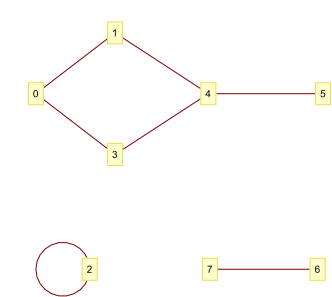
\includegraphics{3.png}\\
\textbf{DepthFirstScan}
\begin{equation*}
0,1,4,5,3
\end{equation*}

\begin{lstlisting}
DepthFirstScan[
Graph[{0 -> 1, 0 -> 3, 1 -> 4, 2 -> 2, 3 -> 4, 4 -> 5, 
6 -> 7}], 0, {"PrevisitVertex" -> (Print["Visiting", #] &)}]
\end{lstlisting}
\textbf{BreadthFirstScan}
\begin{equation*}
0,1,3,4,5
\end{equation*}

\begin{lstlisting}
BreadthFirstScan[
Graph[{0 -> 1, 0 -> 3, 1 -> 4, 2 -> 2, 3 -> 4, 4 -> 5, 
6 -> 7}], 0, {"PrevisitVertex" -> (Print["Visiting", #] &)}]
\end{lstlisting}
\textbf{Choice of algorithm}
\begin{itemize}
	\item Here, we could use both the matrix form or list form. Both will do. That is because we have twice as many vertices as edges, so approx. one path between each edge. For memory, my gut feeling suggests the list form as the matrix one has many zeros (and we have few vertices).
	\item Here, as we deal with many vertices(in the order of a $10^4$), there are going to be many more paths, so better to use matrix form. \color{blue}Correction: List is still better. A matrix would have $1000\times1000 =10^6 $ items, and removing the edges would still leave $950000$ zeros. \color{black}
	\item List is better because we can easily look up a certain combination.
\end{itemize}
\textbf{Theta $n^2$}\\
On one hand, this is strange since all neighbours are in the same row, so it should be fast. But, the problem is actually in the recursion. Each time, we are going to look up neighbours' neighbours, which requires us to jump to different rows and go through them. We are going to load the same row more than once.

\section*{HashGraph}
\lstinputlisting{Graph/src/kth/csc/inda/HashGraph.java}

\section*{Random Graphs}

\subsection*{Different trials, n=1000..5000}

% Table generated by Excel2LaTeX from sheet 'Sheet1'
\begin{table}[htbp]
  \centering
  \caption{Results}
    \begin{tabular}{rrr}
    \hline
    HashGraph & MatrixGraph & HashGraph-MatrixGraph \\
    \hline
    705292 & 1670450 & -965158 \\
    676144 & 966390 & -290246 \\
    318982 & 938473 & -619491 \\
    220044 & 1530869 & -1310825 \\
    247960 & 1541543 & -1293583 \\
    \hline
    \end{tabular}%
  \label{tab:addlabel}%
\end{table}%

\subsection*{Result when n=1000}
\begin{verbatim}
The graph consists of 907 components.
The longest one is located at 940 with the size of 94 items.
\end{verbatim}
\subsection*{Conclusion}
To sum up, HashGraph seems to be faster on average than MatrixGraph. There appears to be an increasing difference in speed as graphs get bigger (HashGraph will be the fastest one).

\subsection*{Rand class}
\lstinputlisting{Graph/src/kth/csc/inda/Rand.java}

\subsection*{Stopwatch}
\lstinputlisting{Graph/src/kth/csc/inda/Stopwatch.java}

\end{document}

